%!TEX root = ../report.tex
\documentclass[report.tex]{subfiles}
\begin{document}
    \chapter{Introduction}
    In the field of industrial robotics, achieving high levels of accuracy, precision, and repeatability in free-space motion is a critical requirement. To meet this requirement, robots must be designed to be stiff and avoid contact along their trajectories. One approach to achieving a high degree of stiffness is to use lightweight materials such as carbon fibre. However, the production of carbon fiber is expensive, leading some companies to opt for cheaper and heavier robot manipulators to reduce manufacturing costs. While this approach may reduce costs, it also results in increased energy consumption as the robot must expend more energy to maintain its joints and links in mid-air.

    During motion planning, robot manipulators commonly treat contact surfaces as obstacles rather than opportunities. This approach contrasts with the behaviour of humans. Take a writing task as an example, as human we often rest our wrists on a table while writing on paper as figure \ref{human_write} shows, however, robot tends to maintain their end effector in midair as figure \ref{robot_write} shows.  By exploiting contact surfaces, robots can achieve selective improvements in accuracy and precision compared to writing on paper with their wrists in mid-air. Furthermore, utilising contact surfaces can help reduce energy consumption.
    
     \begin{figure}[H]
        \captionsetup[figure]{justification=centering}
        \begin{subfigure}{0.49\textwidth}
                \centering
                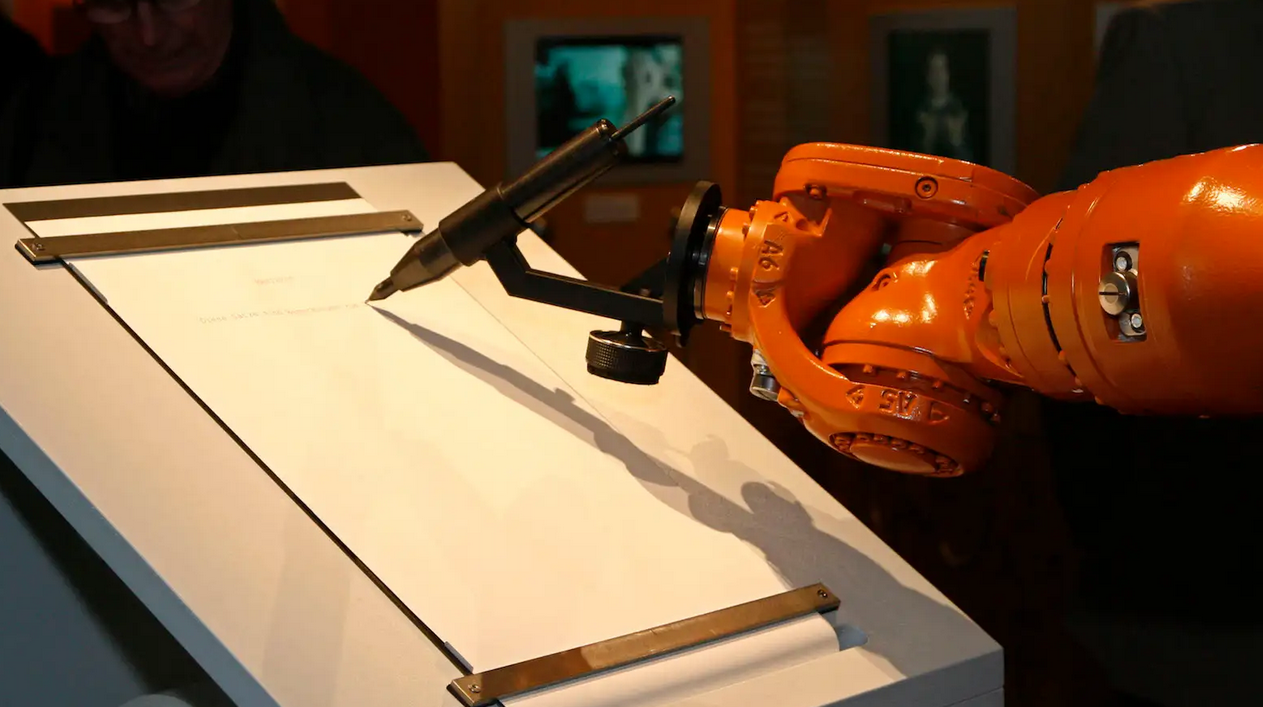
\includegraphics[width=\linewidth]{images/robot_write.png}
                \caption{The example of robot performing writing \cite{Newton_2017}}
                \label{robot_write}
            \end{subfigure}
            \begin{subfigure}{0.49\textwidth}
                \centering
                
\includegraphics[width=\linewidth]{images/human_write.jpg}
                \caption{Picture of human writing \cite{Says_2022}}
                \label{human_write}
            \end{subfigure}
            \caption{The comparison of robot and human performing writing task}
    \end{figure}


    To enable robots to imitate this behaviour, two adaptations of control software are required: Dynamics and partial constraint. Contact handling requires not only the kinematics of the robot but also its dynamics. There are existing dynamic solvers that can be used to solve the robot’s equations of motion. To fully exploit the contact surface, the specification of partial constraints must be introduced. The acceleration-constrained hybrid dynamics algorithm (ACHDA) limits the ability to handle the partial constraint of an end-effector. ACHDA can handle partial motion specifications in some direction and leave them determined by nature. Since nature determines part of the motion, the solver provides higher energy efficiency, passive adaptation, and desire constraints that do not require explicit control. Shakhimardanov has demonstrated the potential for extending constraints to arbitrary links \cite{Shakhimardanov2015}. However, this extension has not yet been incorporated into any software library. This means that while the theoretical framework for extending constraints to arbitrary links has been established, it has not yet been implemented in practice
    
    In this research and development project, we will address three case studies to demonstrate a robot that exploits environmental constraints: Grasping an object by sliding along its surface, performing a writing task, and resting robot manipulation. The first case study aims to establish the required infrastructure for task execution through a proof-of-concept task. The second case study aims to implement the extension of the Vereshchagin solver in daily tasks to investigate whether exploiting contact surfaces can improve the accuracy and precision of robot motion. The third case study aims to evaluate whether resting some of the joints on a supporting surface can lead to higher energy efficiency.

    The content of this research and development report is presented as follows. First, the State of the art will be introduced in chapter \ref{State of the Art} to deliver a brief idea on the related work in dynamics, controllers, a stack of tasks, and some related work. From the deficits of the existing state of the art, chapter \ref{Background} will describe the core of this research and development project, Popov-Vereshchagin (PV) solver, especially the task interface of the PV solver. In the software development side, KDL library provides a function to aid the computation of differences between a variety kinds of data structures by using function overloading. After giving a concrete idea of the background of the PV solver and the robot interface, in chapter \ref{Solution}, robot architecture is proposed. It consists of two major parts: a cascaded controller to control the $\beta$ value mentioned in \ref{Background} and the PV solver. Then the extension of Robif2b, a robot control interface, is introduced as it shows the flexibility such that we can selectively choose what port we can communicate with the robot. Then the experiment design, setup, and evaluation will be delivered in chapter \ref{exp} on a use case basis where three use cases: (1) Grasp object by sliding motion along surface (2) Perform writing task and (3) Resting elbow manipulation will be investigated. In the end, a conclusion will be given, to sum up the project and proposed possible future work.
    
\end{document}